
\documentclass{article}
\usepackage[utf8]{inputenc}
\usepackage[T1]{fontenc}
\usepackage{geometry}
\usepackage{amsmath}
\usepackage{amssymb}
\geometry{a4paper}
\title{The evolution of mobile data thecnologies, from 2G to 5G\\
	\large Tema da trabalho \\}
\author{André Melo, Rafael Lima e Rodrigo Anciães}
%\date{data}
\begin{document}

\maketitle
\begin{abstract}
Mobile communications technologies utilize radio frequencies to be able to perform a range of different things, from voice calls to content drastically changed the way mobile data is transmitted.
\end{abstract}
\pagebreak

\section{2G and it's innovations over previous mobile data technologies}
2G's innovations over it's predecessors lay in it's use of digital signals instead of analogue. While 1G used frequency modulation at a band of band of 824-894MHz to encode information, 2G used mostly TDMA and CDMA for it's modulation schemes and had a bitrate of 64kbps, and a bandwith of 30-200KHz. While TDMA has only a single channel, that allocates timeslots for each user transmitting data, CDMA dealt with user signal division by giving each user an uniquely ID'd channel(citation needed). Since it's signals are digital, cellphone communication technologies other than phone calls became possible, such as the SMS. 2G's most widely used modulation scheme whowever, GSM (Global System for Mobile Communication), used a mix of TDMA and FDMA. It's total bandwith was divided into multiple frequency channels, and each channel was then divided using the TDMA scheme[1]

\section{3G's incremental approach to improving 2G}
While 2G's innovations over it's predecessors where massive, the process of innovation from 2G to 3G was much more incremental. 3G's purpose is to serve as an improved version of 2G, with faster data transfer speeds of up to 2Mbps, while having a frequency band of 15-20MHz, making it's use possible for applications such as web browsing and other more data heavy applications.

\section{4G}

\section{5G and the creation of new structures and capabilitys}
\paragraph{}
Differently, from some of its predecessors, 5G aims to be a massive step forward its predecessors focusing on causing a revolutionary impact in terms of data rates, latency, massive connectivity, network reliability, and energy efficiency, creating the need and creating a way to new data transmission structures.\par
\subsection*{5G's new structures}
\paragraph{}
Another step forward made by 5G is the transition from cell centricity to device centricity which exploits and harnesses intelligence at the device side (human or machine) such as via device-to-device (D2D) communication of UE-assisted mobility [3].\par
Due to the saturation of the already-in-use frequency bands and its consequent lack of bandwidth, 5G is targeting the frequency band in the mm-wave range from 24-100 GHz, creating, due to its approval, a new communication-only band.\par
In addition to 5G new structures, massive MIMO stands out as a key enabling capability. Also called MU-MIMO, it is a significantly enhanced form of MIMO technology that uses a collection of antennas orchestrated to concurrently serve multiple tens of UEs using a one-time frequent slot i.e. same time-frequency resource [3]. Also, the high frequency in that 5G operates, makes it possible to deploy large-scale antenna arrays at the base station, which are used to provide array gain to overcome higher path loss and provide spatial multiplexing gain [2].\par
\subsection*{5G's some conterpoints to the 5G use}
\paragraph{}
Besides its advances and benefits, the 5G technology has unavoidable problems in transmission as higher attenuation and dispersion than its predecessors.\par
Since mm-waves do not effectively penetrate or diffract around, one of the most relevant cases of attenuation is the case of attenuation due to outdoor to indoor penetration, which can impose losses up to 20-40 dB (may be seen in Fig 1).\par
\begin{figure}[h]
\centering
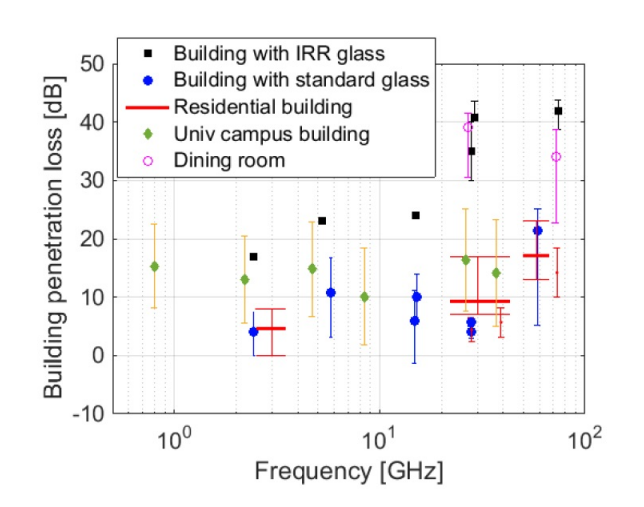
\includegraphics[width=0.5\textwidth]{Fig1.png}
\caption{Attenuation due to outdoor to indoor penetration}
\end{figure}
Another case of attenuation caused by the same motives is the one caused by the shadowing of objects and people, which can cause losses of up to 20 dB.\par
\subsection*{5G data rates}
\paragraph{}
Besides the vulnerability to attenuation and pathloss, 5G still makes a solid step forward in data rate, being up to 1Tbps theoretically, though this volume is just expected to be achieved by 2030. Meanwhile, peak data rates over 10Gbps may be achieved in specific scenarios such as indoor and dense outdoor environments, in this case, A range of 10-50Gbps can be achieved for low mobility users, with ≥ 100Mbps cell-edge data rate guaranteed for 95% of the users [1].\par
Also, It is worth noting that the IMT-2020 has set minimum requirements for peak data rates in a workable 5G network to be 20Gbps and 10Gbps in the DL and UL respectively [1].\par
\section

\section{References}
[1]Javier Gozálvez Sempere"An overview of the GSM system"
[2]Mansoor Shafi, Andreas F. Molisch, Peter J Smith, Thomas Haustein, Peiying Zhu, Prasan De Silva, Fredrik
Tufvesson, Anass Benjebbour, Gerhard Wunder"5G: A Tutorial Overview of Standards, Trials, Challenges, Deployment and Practice"
[3]Opeoluwa Tosin Eluwole, Nsima Udoh, Mike Ojo, Chibuzo Okoro and Akintayo Johnson Akinyoade "From 1G to 5G, What Next?"

\end{document}